\documentclass{article}
\usepackage{setspace}
\usepackage{amsfonts}
\usepackage{graphicx}
\usepackage{amsmath}
\graphicspath{{./figures/}}

\title{Heterogeneous multiscale modeling of plasma confined to a two-dimensional periodic domain}
\author{Jeffrey Haack, Michael Murillo, Jacob Price, Gil Shohet}


\begin{document}

\maketitle

\begin{abstract}
Plasma modeling can be conducted with varying levels of detail. The Bhatnagar-Gross-Krook approximation is an effective kinetic model for hot plasma given an accurate relaxation parameter. This parameter, however, is difficult to know \emph{a priori}. Molecular dynamics offers a fully detailed model for ionic motion. The heterogeneous multiscale method (HMM) provides a computational and analytical link between disparate physical models. In this paper, we present a proof of concept of HMM as a modeling method for hot plasma. The unknown relaxation parameter can be computed from short molecular simulations, and then used in subsequent kinetic time steps. Simulations using the hybrid kinetic-molecular dynamic model are both more accurate than the kinetic model alone, and orders of magnitude more efficient than the molecular dynamics model alone. The HMM philosophy can be used similarly to hybridize physical models in a way that creates a stark improvement over both original models.
\end{abstract}

\section{Introduction}

Many mathematical and scientific problems contain phenomena at widely different scales. Multiscale modeling aims to take advantage of this disparity to understand complex behavior at each level of detail \cite{weinan2011principles}. Multiphysics problems are a prototypical example of problems that are well-addressed by a multiscale approach. There is a hierarchy of physical models of varying levels of detail and coarseness. Quantum mechanics (QM) provides a complete description of physical interactions, but is often computationally and analytically intractable for all but the simplest systems. From quantum mechanics, one can derive laws of molecular dynamics (MD) as a more tractable, but less detailed physical description than the wave functions of QM. From MD, kinetic theory (KT) can be derived as a statistical description of molecular motion. An even coarser model, hydrodynamics, can be derived either directly from MD or from KT.

With each step up in the hierarchy, physical detail is sacrificed for intuition and computational tractability. In reality, these levels of detail form a continuum, rather than classes of problems. Hydrodynamics describe bulk motion well, unless that motion involves a crack in the material, or a propagating shock. In these regions of interest, kinetic effects, or even molecular effects cannot be disregarded. In this way, multiphysics and multiscale modeling become important in different regions of interest.

Often coarser models contain parameters that can be interpreted as averaged quantities from higher detail models. For example, stress tensors in hydrodynamics can be computed from the second velocity moment of a kinetic description of the same system. When one confines oneself to a coarse model, these parameters can prove difficult. These parameters are precomputed as a function of macroscopic variables and tabulated in a reference table for use in all later simulations. One major limitation is the fact that we may be unable to anticipate all relevant arrangements. It would be better to be able to compute these parameters accurately ``on the fly.''

This leads to the concept of the heterogeneous multiscale method (HMM) \cite{weinan2007heterogeneous}. HMM takes a top-down approach to multiphysics modeling. Two (or more) levels of physical detail are selected, such that the analysis and computation could be completed in any level and yield consistent results. HMM focuses on the coarsest model, as this is one can be computed efficiently over a much larger time scale than the more detailed model. This coarse model, as discussed above, contains parameters that are averaged quantities from the higher-detail model. The general approach is to spend most computational time in the coarse regime, periodically down sampling to the fine regime to use brief simulations to recompute parameters used in the coarse regime. The result is a hybrid simulation method that contains the computational speed of the coarse model with highly accurate parameters drawn from the fine model. The proposed method is illustrated in Figure \ref{HMM}.



\begin{figure}[h]\begin{center}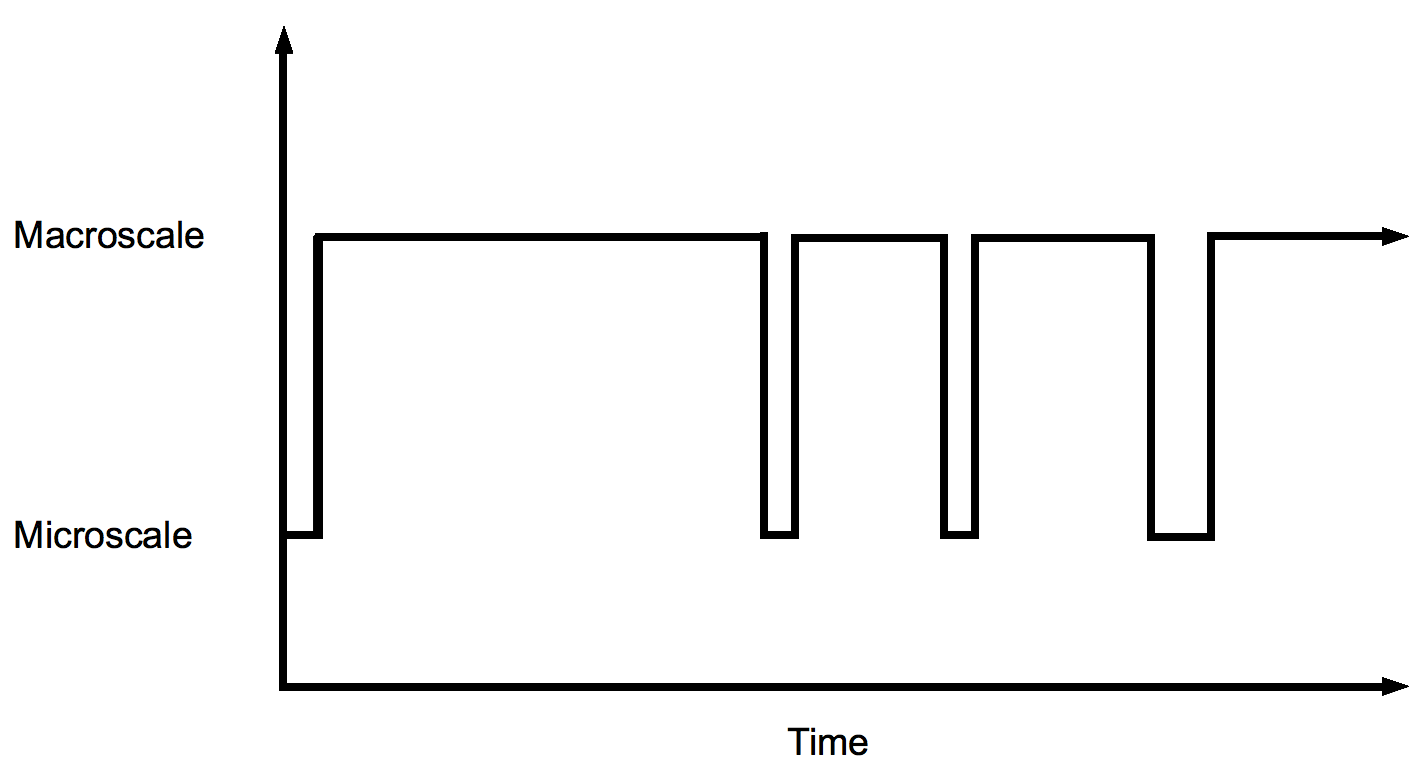
\includegraphics[width=.6\linewidth]{scheme.pdf}\caption{A cartoon of the computational time spent in different computational regimes during an HMM simulation.}\label{HMM}\end{center}\end{figure}

The structure of this paper will be as follows. In Section 2, we will describe the system of interest and the selected physical regimes, along with their governing equations. In Section 3, we rigorously connect the fine grain description to the coarse grain description, and in doing so demonstrate the exact nature of the connecting parameters. We also rigorously rationalize simplifying decisions made in the modeling steps. In section 4, we make explicit the manner in which we transition between levels of detail. In practice, this is the most difficult part of HMM. In Section 5, we non-dimensionalize both models to isolate interesting timescales and improve numerical computations. In Section 6, we present the results of our computations, comparing fully fine-grained simulations with hybrid HMM simulations. We comment on insights that can be gleaned from the longer time scale the HMM method allows us to study. Finally, in Section 7, we comment on the possibilities and downsides of this scheme for this specific problem and similar classes of problems.

\section{Plasma modeling}

Plasma is a dense, electrically neutral system of charged ions and electrons, in which each ion interacts with many neighbors, making collective effects critical \cite{sturrock1994plasma}. This near-neighbor interaction is represented by the \emph{Debye length} $\lambda$. Because opposite charges attract, each positive ion tends to be surrounded by several negatively charged electrons, which effectively ``screen'' the electrostatic field due to the other particles. Plasma particles only significantly interact with other particles within one Debye length. Other interactions drop off due to the strong length dependence on forces, and an effective ``screening'' by background electrons. Examples of plasmas include astrophysical phenomena such as stars and the interplanetary medium, terrestrial phenomena such as lightning and aurorae, and technological constructs such as plasma televisions and material used in fusion reactor research.

Our system of interest is hot plasma in which the ions are confined to a two-dimensional plane on a periodic domain. Periodic boundary conditions effectively represent the behavior of a much larger domain, since particle interactions are screened by the Debye length. Particles are only affected by their nearest neighbors. One reason we confine ourselves to two-dimensional simulation is computational efficiency. We seek to demonstrate multiscale plasma modeling through a proof of concept. All of the conclusions and methods described in this paper can be extended to more complicated systems with little difficulty. Additionally, there are physical examples of plasmas that are confined to a plane. \emph{Dusty plasmas} consist of large (millimeter to nanometer), charged particles. They can be found in the mesosphere of the earth, industrial processing, and laboratory experiments. In experiments, they can be confined to a plane by a balance of gravitational force and electric force from a vertical lab-generated electric field. Electrons, which weigh far less than the ions, are free to move in three dimensions, but the motion of the ions is confined to a flat plane \cite{shukla2001introduction}.

In order to use HMM to simulate this system, we select the Bhatnagar-Gross-Krook (BGK) approximation of the Boltzmann equation of kinetic theory as our coarse model and molecular dynamics as our fine model. The quantity of interest in the BGK model is the distribution of particles $f(\mathbf{r},\mathbf{p})$ which gives the density of particles at position $\mathbf{r}=(x,y)$ with momentum $\mathbf{p}=(p_x,p_y)$. The partial differential equation governing this distribution is
\begin{equation}
\begin{split}
&\frac{f_{eq}-f}{\tau}=\frac{\partial f}{\partial t}+\frac{\mathbf{p}}{m}\cdot \nabla_\mathbf{r} f-\frac{q}{m}\nabla_\mathbf{r}\phi\cdot\nabla_\mathbf{p}f\\
&\nabla^2_\mathbf{r}\phi=-\frac{e}{\epsilon_0}\left(n(\mathbf{r})-n_{e_0}-\frac{en_{e_0}}{k_BT_e}\phi\right)\\
&f(\mathbf{r},\mathbf{p},0)=f_0(\mathbf{r},\mathbf{p})\\
&f(\mathbf{r},\mathbf{p},t)_{x=0}=f(\mathbf{r},\mathbf{p},t)_{x=L_x},\;\;\;\;
f(\mathbf{r},\mathbf{p},t)_{y=0}=f(\mathbf{r},\mathbf{p},t)_{y=L_y}\\
&\phi(\mathbf{r},t)_{x=0}=\phi(\mathbf{r},t)_{x=L_x},\;\;\;\;\;\;\;\;\;\;\;\;
\phi(\mathbf{r},t)_{y=0}=\phi(\mathbf{r},t)_{y=L_y}
\end{split}\label{eq:BGK}
\end{equation}Here, $q$ is the charge of the ion and $m$ is its mass. $f_{eq}$ is the equilibrium distribution of the ion, and $\tau$ is a relaxation time. $\phi$ is the electric potential, described by the second equation. This is a linearized version of the nonlinear Poisson's equation using the Boltzmann relation. See Section 3 for the derivation of this expression. $e$ is the unit charge, $n(\mathbf{r})$ is the density of ions, which is defined as $n(\mathbf{r})=\int f\, d\mathbf{p}$, $\epsilon_0$ is the medium's electrical permittivity, $k_B$ is Boltzmann's constant, $T_e$ is the temperature of the background electrons. $n_{e_0}$ is a constant parameter guaranteeing global charge neutrality, $n_{e_0}=\int n(\mathbf{r})\,d\mathbf{r}$. If there are multiple species of ions, with their own unique masses $m_i$, charges $q_i$, and distributions $f_i$, they are each evolved according to their own PDE as in equation one, with the same boundary conditions. The differential equation for Poisson's equation remains the same, but the particle density $n(\mathbf{r})=\sum_i n_i(\mathbf{r})$.

In the fine MD model, ions are individually tracked according to the Hamiltonian equations
\begin{equation}
\begin{split}
\frac{\partial \mathbf{r}_i}{\partial t}&=\nabla_{\mathbf{p}_i} H\\
\frac{\partial \mathbf{p}_i}{\partial t}&=-\nabla_{\mathbf{r}_i}H\\
H(\mathbf{r}_i,\mathbf{p}_i)&=\sum_i\frac{|\mathbf{p}_i|^2}{2m_i}+\sum_{i<j}U'(\mathbf{r}_i-\mathbf{r}_j)+\sum_i U''\left(\mathbf{r}_i,\{\mathbf{r}_j\}_{j=1}^n\right).
\end{split}\label{eq:MD}
\end{equation}Here $\mathbf{r}_i$ and $\mathbf{p}_i$ are the position and momentum of ion $i$. $H$ is the Hamiltonian of the system, consisting of the sum of the kinetic energy and the potential energy. The potential energy of the system comes from two sources: interparticle potentials defined by $U'(\mathbf{r}_i-\mathbf{r}_j)$ and potential due to the background electrons, which depends upon the spatial arrangement of the ions, $U''\left(\mathbf{r}_i,\{\mathbf{r}_j\}_{j=1}^n\right)$. Ions evolve according to these simple equations in a periodic two-dimensional box. Note that, though motion is confined to this two dimensional box, we assume our system is actually three-dimensional, as in the dusty plasma experiments. Indeed, the electrons are able to move freely in 3D space; only the ions are confined. Note that the existence of different ion species with their own masses and charges pose no additional complications on this model. A fully detailed description in this regime would include the Hamiltonian equations for the motion of the electrons, however for simplicity we do not track the electrons individually. We only monitor their collective effects on each ion. In the next section, we will illustrate the connection between these two physical descriptions of the same system.

\section{Multiphysics connection}
Our system is described in full detail when we evolve every ion in the molecular dynamics simulation according to the Hamiltonian equations (\ref{eq:MD}). We will derive, from this starting point, the BGK kinetic theory formulation of the problem (\ref{eq:BGK}). We construct an indicator function that stores the location $\mathbf{r}_i$ and momentum $\mathbf{p}_i$ of every ion at a given time $t$:
\begin{equation}N(\mathbf{r},\mathbf{p},\{\mathbf{r}_i\}_{i=1}^n,\{\mathbf{p}_i\}_{i=1}^n,t)=\sum_i\delta\left(\mathbf{r}-\mathbf{r}_i(t)\right)\delta\left(\mathbf{p}-\mathbf{p}_i(t)\right).
\end{equation}$\delta(x)$ is the Dirac delta function. We are interested in the time evolution of this indicator function. Thus, an aside relating to distributions and their derivatives is warranted

\subsection{Distributional derivatives}
Consider the set of test functions, $D(\mathbb{R})$ that are infinitely differentiable and have compact support. A distribution is a linear mapping $T: D(\mathbb{R})\to\mathbb{R}$. By convention, the operation of a distribution $T$ on a target function $f$ is written $\langle T,f\rangle$. The Dirac delta ``function'' can thus be written $\langle \delta,f\rangle=f(0)$.

The derivative of a distribution is defined as $\langle T',f\rangle=-\langle T,f'\rangle$. This is a consequence of integration by parts:
\begin{eqnarray*}
\langle T',f\rangle=\int_{-\infty}^\infty \delta'(x)f(x)\;dx=\left[f(x)\delta(x)\right]_{-\infty}^\infty-\int_{-\infty}^\infty \delta(x)f'(x)\;dx=-\langle T,f'\rangle
\end{eqnarray*}We discount the first term in the integration by parts because our test functions are considered equal to zero outside of a bounded set. Thus, by this definition, the derivative of the Dirac delta function operating on a function $f$ would simply be:
\[\frac{d}{dx}(\delta(f(x)))=-f'(0).
\]Though we will not explicitly compute this derivative, it suffices to show that it exists and is well-defined. The above definition of the distributional derivative in terms of transferring derivatives from the distribution to the internal function also allows for a seamless use of the product and chain rules in their standard forms in the presence of distributions.  Our problem utilizes two-dimensional Dirac delta functions, defined as
\[\delta(\mathbf{r})=\delta(r_x)\delta(r_y).
\]The gradient of this function similarly exists:
\begin{eqnarray*}
\nabla_\mathbf{r}\delta(\mathbf{r})=\left(\delta(r_y)\frac{d}{dr_x}\delta(r_x),\delta(r_x)\frac{d}{dy}\delta(r_y)\right).
\end{eqnarray*}Gradients of two-dimensional delta functions are thus well defined. We will make use of a useful identity relating to derivatives of delta functions. Recall that the argument of the delta functions used in $N$ took the form $\mathbf{f}=\mathbf{a}-\mathbf{b}$. Consider the Dirac delta gradient with respect to each variable:
\begin{align*}
\nabla_\mathbf{a}\delta(\mathbf{a}-\mathbf{b})&=\left(\delta(a_y-b_y)\langle \delta_{a_x},a_x-b_x\rangle,\delta(a_x-b_x)\langle \delta_{a_y},a_y-b_y\rangle\right)\\
&=\left(-\delta(a_y-b_y)\left\langle\delta,\frac{\partial}{\partial a_x}(a_x-b_x)\right\rangle,-\delta(a_x-b_x)\left\langle\delta,\frac{\partial}{\partial a_y}(a_y-b_y)\right\rangle\right)\\
&=(-\delta(a_y-b_y),-\delta(a_x-b_x))\\
\nabla_\mathbf{b}\delta(\mathbf{a}-\mathbf{b})&=\left(\delta(a_y-b_y)\langle \delta_{b_x},a_x-b_x\rangle,\delta(a_x-b_x)\langle \delta_{b_y},a_y-b_y\rangle\right)\\
&=\left(-\delta(a_y-b_y)\left\langle\delta,\frac{\partial}{\partial b_x}(a_x-b_x)\right\rangle,-\delta(a_x-b_x)\left\langle\delta,\frac{\partial}{\partial b_y}(a_y-b_y)\right\rangle\right)\\
&=(\delta(a_y-b_y),\delta(a_x-b_x))
\end{align*}From this, we see we can make the convenient substitution:
\begin{equation}
\nabla_{\mathbf{r}_i}\delta(\mathbf{r}-\mathbf{r}_i)=-\nabla_\mathbf{r}\delta(\mathbf{r}-\mathbf{r}_i)\label{delderivswitch}
\end{equation}
\subsection{Derivation of BGK}
Returning our attention to the time evolution of the indicator function $N$:
\begin{align*}
\frac{\partial N}{\partial t}=\sum_i& \frac{\partial}{\partial t}\left[\delta(\mathbf{r}-\mathbf{r}_i(t))\delta(\mathbf{p}-\mathbf{p}_i(t))\right]\\
=\sum_i& \delta(\mathbf{p}-\mathbf{p}_i(t))\frac{\partial}{\partial t}\delta(\mathbf{r}-\mathbf{r}_i(t))+\delta(\mathbf{r}-\mathbf{r}_i(t))\frac{\partial }{\partial t}\delta(\mathbf{p}-\mathbf{p}_i(t))\\
=\sum_i&\bigg\{\delta(\mathbf{p}-\mathbf{p}_i(t))\frac{\partial(\mathbf{r}-\mathbf{r}_i(t))}{\partial t}\cdot\nabla_{(\mathbf{r}-\mathbf{r}_i)}[\delta(\mathbf{r}-\mathbf{r}_i(t))]\\
&+\delta(\mathbf{r}-\mathbf{r}_i(t))\frac{\partial(\mathbf{p}-\mathbf{p}_i(t))}{\partial t}\cdot\nabla_{(\mathbf{p}-\mathbf{p}_i)}[\delta(\mathbf{p}-\mathbf{p}_i(t))]\bigg\}\\
=\sum_i&\bigg\{\delta(\mathbf{p}-\mathbf{p}_i(t))(-1)\frac{\partial \mathbf{r}_i(t)}{\partial t}\cdot\nabla_{(\mathbf{r}-\mathbf{r}_i)}[\mathbf{r}_i]\cdot\nabla_{\mathbf{r}_i}[\delta(\mathbf{r}-\mathbf{r}_i(t))]\\
&\delta(\mathbf{r}-\mathbf{r}_i(t))(-1)\frac{\partial \mathbf{p}_i(t)}{\partial t}\cdot\nabla_{(\mathbf{p}-\mathbf{p}_i)}[\mathbf{p}_i]\cdot\nabla_{\mathbf{p}_i}[\delta(\mathbf{p}-\mathbf{p}_i(t))]\bigg\}\\
=\sum_i&\bigg\{\delta(\mathbf{p}-\mathbf{p}_i(t))(-1)\frac{\partial \mathbf{r}_i(t)}{\partial t}(-1)(-1)\cdot\nabla_{\mathbf{r}}[\delta(\mathbf{r}-\mathbf{r}_i(t))]\\
&\delta(\mathbf{r}-\mathbf{r}_i(t))(-1)\frac{\partial \mathbf{p}_i(t)}{\partial t}(-1)(-1)\cdot\nabla_{\mathbf{p}}[\delta(\mathbf{p}-\mathbf{p}_i(t))]\bigg\}\\
=\sum_i&\bigg\{-\frac{\partial \mathbf{r}_i(t)}{\partial t}\delta(\mathbf{p}-\mathbf{p}_i(t))\cdot \nabla_\mathbf{r}[\delta(\mathbf{r}-\mathbf{r}_i(t))]\\&-\frac{\partial \mathbf{p}_i(t)}{\partial t}\delta(\mathbf{r}-\mathbf{r}_i(t))\cdot \nabla_\mathbf{p}[\delta(\mathbf{p}-\mathbf{p}_i(t))]\bigg\}.
\end{align*}We used (\ref{delderivswitch}) in the last step. Here we use the definition of the Hamiltonian to make some substitutions. Assume now that we focus our attention only to one particle species (such that all particles have the same mass $m$). These particles will still interact with other species through the potential function. An identical derivation proceeds for each particle species, yielding a BGK PDE for each species. Consider the partial derivatives we encountered in the above calculation:
\begin{equation}
\frac{\partial \mathbf{r}_i}{\partial t}=\nabla_{\mathbf{p}_i}H=\nabla_{\mathbf{p}_i}\left(\sum_i \frac{|\mathbf{p}_i|^2}{2m}+\sum_{i<j}U'(\mathbf{r}_i-\mathbf{r}_j)+\sum_i U''\left(\mathbf{r}_i,\{\mathbf{r}_j\}_{j=1}^n\right)\right)=\frac{\mathbf{p}_i}{m}\label{dridt},
\end{equation}and
\begin{equation}
\frac{\partial \mathbf{p}_i}{\partial t}=-\nabla_{\mathbf{r}_i}H=-\nabla_{\mathbf{r}_i}\left(\sum_i \frac{|\mathbf{p}_i|^2}{2m_i}+\sum_{i<j}U'(\mathbf{r}_i-\mathbf{r}_j)+\sum_i U''\left(\mathbf{r}_i,\{\mathbf{r}_j\}_{j=1}^n\right)\right)=-\nabla_{\mathbf{r}_i} U\left(\mathbf{r}_i,\{\mathbf{r}_j\}_{j\neq i}\right).\label{dpidt}
\end{equation}$U\left(\mathbf{r}_i,\{\mathbf{r}_j\}_{j\neq i}\right)$ is the potential field at $\mathbf{r}_i$ due to all other ions (and the background electrons). Using (\ref{dridt}) and (\ref{dpidt}),
\begin{align*}
\frac{\partial N}{\partial t}=&\sum_i-\frac{\partial \mathbf{r}_i(t)}{\partial t}\delta(\mathbf{p}-\mathbf{p}_i(t))\cdot \nabla_\mathbf{r}[\delta(\mathbf{r}-\mathbf{r}_i(t))]-\frac{\partial \mathbf{p}_i(t)}{\partial t}\delta(\mathbf{r}-\mathbf{r}_i(t))\cdot \nabla_\mathbf{p}[\delta(\mathbf{p}-\mathbf{p}_i(t))]\\
=&\sum_i-\frac{\mathbf{p}_i}{m}\delta(\mathbf{p}-\mathbf{p}_i(t))\cdot\nabla_\mathbf{r}\delta(r-\mathbf{r}_i(t))+\delta(\mathbf{r}-\mathbf{r}_i(t))\nabla_{\mathbf{r}_i}U\left(\mathbf{r}_i,\{\mathbf{r}_j\}_{j\neq i}\right)\cdot \nabla_\mathbf{p}\delta(\mathbf{p}-\mathbf{p}_i(t)).
\end{align*}
Notice that $\frac{\mathbf{p}_i}{m}\delta(p-p_i(t))$ is only nonzero when $\mathbf{p}=\mathbf{p}_i$, such that 
\begin{equation*}\frac{\mathbf{p}_i}{m}\delta(\mathbf{p}-\mathbf{p}_i(t))=\frac{\mathbf{p}}{m}\delta(\mathbf{p}-\mathbf{p}_i(t)).\end{equation*} 
Similarly, $\nabla_{\mathbf{r}_i}U\left(\mathbf{r}_i,\{\mathbf{r}_j\}_{j\neq i}\right)$ depends on $\mathbf{r}_i$, so $\nabla_{\mathbf{r}_i}U(\mathbf{r}_i)\delta(\mathbf{r}-\mathbf{r}_i(t))$ is only nonzero when $\mathbf{r}=\mathbf{r}_i$, at which point \begin{equation*}\nabla_{\mathbf{r}_i}U\left(\mathbf{r}_i,\{\mathbf{r}_j\}_{j\neq i}\right)\delta(\mathbf{r}-\mathbf{r}_i(t))=\nabla_\mathbf{r}U\left(\mathbf{r},\{\mathbf{r}_j\}_{j=1}^n\right)\delta(\mathbf{r}-\mathbf{r}_i(t))\end{equation*}with the definition that the potential due to a ion at its own position is zero. Making these substitutions,
\begin{align*}
\frac{\partial N}{\partial t}=&\sum_i-\frac{\mathbf{p}_i}{m}\delta(\mathbf{p}-\mathbf{p}_i(t))\cdot\nabla_\mathbf{r}\delta(\mathbf{r}-\mathbf{r}_i(t))+\delta(\mathbf{r}-\mathbf{r}_i(t))\nabla_{\mathbf{r}_i}U\left(\mathbf{r}_i,\{\mathbf{r}_j\}_{j\neq i}\right)\cdot \nabla_\mathbf{p}\delta(\mathbf{p}-\mathbf{p}_i(t))\\
\frac{\partial N}{\partial t}=&\sum_i-\frac{\mathbf{p}}{m}\delta(\mathbf{p}-\mathbf{p}_i(t))\cdot\nabla_\mathbf{r}\delta(\mathbf{r}-\mathbf{r}_i(t))+\delta(\mathbf{r}-\mathbf{r}_i(t))\nabla_{\mathbf{r}}U\left(\mathbf{r},\{\mathbf{r}_j\}_{j=1}^n\right)\cdot \nabla_\mathbf{p}\delta(\mathbf{p}-\mathbf{p}_i(t))\\
\frac{\partial N}{\partial t}=&-\frac{\mathbf{p}}{m}\cdot \nabla_\mathbf{r}\left[\sum_i\delta(\mathbf{r}-\mathbf{r}_i(t))\delta(\mathbf{p}-\mathbf{p}_i(t))\right]\\&+\nabla_\mathbf{r}U\left(\mathbf{r},\{\mathbf{r}_j\}_{j=1}^n\right)\cdot\nabla_\mathbf{p}\left[\sum_i\delta(\mathbf{r}-\mathbf{r}_i(t))\delta(\mathbf{p}-\mathbf{p}_i(t))\right]\\
\frac{\partial N}{\partial t}=&-\frac{\mathbf{p}}{m}\cdot\nabla_\mathbf{r} N+\nabla_\mathbf{r} U\left(\mathbf{r},\{\mathbf{r}_j\}_{j=1}^n\right)\cdot \nabla_\mathbf{p}N.
\end{align*}We now take the ensemble average of both sides of this equation, with the definition $f(\mathbf{r},\mathbf{p},t)=E[N]$. This ensemble is taken with respect to all equivalent initial choices for $\mathbf{r}_i(0)$ and $\mathbf{p}_i(0)$. Thus, this expected value only acts on the $\mathbf{r}_i$ and $\mathbf{p}_i$ variables. Using this, we can show:
\begin{align*}
E\left[\frac{\partial N}{\partial t}\right]=&E\left[-\frac{\mathbf{p}}{m}\cdot \nabla_\mathbf{r} N+\nabla_\mathbf{r} U\left(\mathbf{r},\{\mathbf{r}_j\}_{j=1}^n\right)\cdot \nabla_\mathbf{p} N\right]\\
\frac{\partial E[N]}{\partial t}=&-E\left[\frac{\mathbf{p}{m}}\cdot \nabla_\mathbf{r}N\right]+E\left[\nabla_\mathbf{r} U\left(\mathbf{r},\{\mathbf{r}_j\}_{j=1}^n\right)\cdot\nabla_\mathbf{p}N\right]\\
\frac{\partial f}{\partial t}=&-\frac{\mathbf{p}}{m}\cdot\nabla_\mathbf{r}E[N]+E\left[\nabla_\mathbf{r} U\left(\mathbf{r},\{\mathbf{r}_j\}_{j=1}^n\right)\cdot \nabla_\mathbf{p}N\right]\\
\frac{\partial f}{\partial t}=&-\frac{\mathbf{p}}{m}\cdot\nabla_\mathbf{r} f+E\left[\nabla_\mathbf{r} U\left(\mathbf{r},\{\mathbf{r}_j\}_{j=1}^n\right)\cdot\nabla_\mathbf{p}N\right].
\end{align*}Because $\mathbf{p}$ and the $\nabla_\mathbf{r}$ gradient do not depend on any of the ensemble variables, we were able to simplify the first term. We cannot do the same with the second term because the potential field is heavily dependent on the positions of the ions. We will focus our attention on this term for the next section of the analysis. First we separate out the part of the potential that depends on the ensemble from the part of the potential that depends on the background electrons:
\begin{align*}
E\left[\nabla_\mathbf{r} U(\mathbf{r})\cdot\nabla_\mathbf{p}N\right]=&E\left[\nabla_\mathbf{r} \left(\sum_{j}U'(\mathbf{r}-\mathbf{r}_j)+U''\left(\mathbf{r},\{\mathbf{r}_j\}_{j=1}^n\right)\right)\cdot \nabla_\mathbf{p} N\right].
\end{align*}Consider multiplying the potential functions by several delta functions and integrating:
\begin{align*}
\sum_j U'(\mathbf{r}-\mathbf{r}_j)=&\sum_j\int\int U'(\mathbf{r}-\mathbf{r}')\delta(\mathbf{r}'-\mathbf{r}_j)\delta(\mathbf{p}'-\mathbf{p}_j)\,d\mathbf{r}'d\mathbf{p}'\\
=&\int\int U'(\mathbf{r}-\mathbf{r}')\sum_j\delta(\mathbf{r}'-\mathbf{r}_j)\delta(p'-p_j)\,d\mathbf{r}'d\mathbf{p}'\\
=&\int\int U'(\mathbf{r}-\mathbf{r}')N(\mathbf{r}',\mathbf{p}',t)\,d\mathbf{r}'d\mathbf{p}'\\
U''\left(\mathbf{r},\{\mathbf{r}_j\}_{j=1}^n\right)=&\int\cdots\int U''\left(\mathbf{r},\{\mathbf{r}_j\}_{j=1}^n\right)\delta(\mathbf{r}^{(1)}-\mathbf{r}_1)\cdots\delta(\mathbf{r}^{(n)}-\mathbf{r}_n)\delta(p'-p_j)\,d\mathbf{r}^{(1)}\cdots d\mathbf{r}^{(n)}d\mathbf{p}'\\
=&\int\cdots\int U''\left(\mathbf{r},\{\mathbf{r}^{(i)}\}_{i=1}^n\right)\,d\mathbf{r}^{(1)}\cdots d\mathbf{r}^{(n)}d\mathbf{p}'
\end{align*}where we have suppressed writing the dependence of $N$ on the positions and momenta of each ion. Plugging this into our remaining expected value expression,
\begin{align*}
E\left[\nabla_\mathbf{r}\sum_jU'(\mathbf{r}-\mathbf{r}_j)\cdot \nabla_\mathbf{p}N(\mathbf{r},\mathbf{p},t)\right]=&E\left[\nabla_\mathbf{r}\left(\int\int U'(\mathbf{r}-\mathbf{r}')N(\mathbf{r}',\mathbf{p}',t)\,d\mathbf{r}'d\mathbf{p}'\right)\cdot\nabla_\mathbf{p}N(\mathbf{r},\mathbf{p},t)\right]\\
=&E\left[\int\int\nabla_\mathbf{r}U'(\mathbf{r}-\mathbf{r}')N(\mathbf{r}',\mathbf{p}',t)\,d\mathbf{r}'d\mathbf{p}'\cdot\nabla_\mathbf{p}N(\mathbf{r},\mathbf{p},t)\right]\\
=&E\left[\int\int\nabla_\mathbf{r}U'(\mathbf{r}-\mathbf{r}')\cdot\nabla_\mathbf{p} N(\mathbf{r}',\mathbf{p}',t)N(\mathbf{r},\mathbf{p},t)\,d\mathbf{r}'d\mathbf{p}'\right]\\
=&\int\int\nabla_\mathbf{r}U'(\mathbf{r}-\mathbf{r}')\cdot\nabla_\mathbf{p}E\left[N(\mathbf{r},\mathbf{p},t)N(\mathbf{r}',\mathbf{p}',t)\right]\,d\mathbf{r}'d\mathbf{p}'.
\end{align*}We have once again brought the expected value down to the only terms that depend on the ion positions and momenta. Let us consider this term more carefully:
\begin{align*}
N(\mathbf{r},\mathbf{p},t)N(\mathbf{r}',\mathbf{p}',t)=\left(\sum_i\delta(\mathbf{r}-\mathbf{r}_i(t))\delta(\mathbf{p}-\mathbf{p}_i(t))\right)\left(\sum_j\delta(\mathbf{r}'-\mathbf{r}_j(t))\delta(\mathbf{p}'-\mathbf{p}_j(t))\right).
\end{align*}This expression is only nonzero when there is a particle $i$ at $(\mathbf{r},\mathbf{p})$ and a particle $j$ at $(\mathbf{r}',\mathbf{p}')$. Thus, it can be expressed as:
\begin{align*}
N_2(\mathbf{r},\mathbf{p},\mathbf{r}',\mathbf{p}',\{\mathbf{r}_k\}_{k=1}^n,\{\mathbf{p}_k\}_{k=1}^n,t)=\sum_{i,j}\delta(\mathbf{r}-\mathbf{r}_i(t))\delta(\mathbf{p}-\mathbf{p}_i(t))\delta(\mathbf{r}'-\mathbf{r}_j(t))\delta(\mathbf{p}'-\mathbf{p}_j(t))
\end{align*}$N_2$ is a generalization of $N$ to two particles. Its expected value is written as $f_2(\mathbf{r},\mathbf{p},\mathbf{r}',\mathbf{p}',t)$. Unfortunately, we have introduced this new unknown function $f_2$, when we wish to express our kinetic system as a partial differential equation for $f$. Because $f_2$ can be considered a two-particle correlation function, we write it without loss of generality as
\begin{equation}f_2(\mathbf{r},\mathbf{p},\mathbf{r}',\mathbf{p}',t)=f(\mathbf{r},\mathbf{p},t)f(\mathbf{r}',\mathbf{p}',t)+C\label{f2}
\end{equation}where $C$ is a complicated, unknown remainder function. Substituting this into our differential equation, we have
\begin{align*}
E\left[\nabla_\mathbf{r} U(\mathbf{r})\cdot\nabla_\mathbf{p}N\right]=&\int\int\nabla_\mathbf{r}U'(\mathbf{r}-\mathbf{r}')\cdot\nabla_\mathbf{p}[f(\mathbf{r},\mathbf{p},t)f(\mathbf{r}',\mathbf{p}',t)+C]\,d\mathbf{r}'d\mathbf{p}'+\nabla_\mathbf{r}U''(\mathbf{r})\cdot\nabla_\mathbf{p}f\\
=&\nabla_\mathbf{r}\left(\int\int U'(\mathbf{r}-\mathbf{r}')f(\mathbf{r}',\mathbf{p}',t)\,d\mathbf{r}'d\mathbf{p}'\right)\cdot\nabla_\mathbf{p}f+\nabla_\mathbf{r}U''(\mathbf{r})\cdot\nabla_\mathbf{p}f+C'\\
=&\nabla_\mathbf{r}\left(\int\int U'(\mathbf{r}-\mathbf{r}')f(\mathbf{r}',\mathbf{p}',t)\,d\mathbf{r}'d\mathbf{p}'+U''(\mathbf{r})\right)\cdot\nabla_\mathbf{p} f+C'\\
=&\nabla_\mathbf{r}\left(\int U'(\mathbf{r}-\mathbf{r}')\int f(\mathbf{r}',\mathbf{p}',t)\,d\mathbf{p}'d\mathbf{r}'+U''(\mathbf{r})\right)\cdot\nabla_\mathbf{p} f+C'\\
=&\nabla_\mathbf{r}\left(\int U'(\mathbf{r}-\mathbf{r}')n(\mathbf{r}',t)\,d\mathbf{r}'+U''(\mathbf{r})\right)\cdot\nabla_\mathbf{p} f+C'
\end{align*}$C'$ is an additional unknown function relating to the collisional properties of the system. We will address it in the next subsection. We here made use of the fact that the particle density $n(\mathbf{r},t)$ is defined as the momentum integral of $f$. Up until this point, we have left the potential functions $U'(\mathbf{r}-\mathbf{r}')$ and $U''(\mathbf{r})$ undefined. Let $Ze$ be the electric charge of the ion ($Z$ is the charge in units of elementary charge). We define the interparticle interaction to be a Coulomb potential. The response to the background electrons is also a Coulomb potential, but with an as yet undefined electron density $n_e(\mathbf{r},t)$. Though we are confined to two-dimensional motion, our equations exist in three-dimensional space, so the Coulomb potential is proportional to the distance between to charged particles.
\begin{align*}
E\left[\nabla_\mathbf{r} U(\mathbf{r})\cdot\nabla_\mathbf{p}N\right]=&\nabla_\mathbf{r}\left(\int U'(\mathbf{r}-\mathbf{r}')n(\mathbf{r}',t)\,d\mathbf{r}'+U''(\mathbf{r})\right)\cdot\nabla_\mathbf{p} f+C'\\
=&\nabla_\mathbf{r}\left(\int \frac{Z^2e^2}{4\pi\epsilon_0|\mathbf{r}-\mathbf{r}'|}n(\mathbf{r}',t)\,d\mathbf{r}'-\int \frac{Ze}{4\pi\epsilon_0|\mathbf{r}-\mathbf{r}'|}en_e(\mathbf{r}',t)dr'\right)\cdot\nabla_\mathbf{p}f+C'
\end{align*}We define the charge density of the ions as $\rho(\mathbf{r},t)=Zen(\mathbf{r},t)$, so
\begin{align*}
E\left[\nabla_\mathbf{r} U(\mathbf{r})\cdot\nabla_\mathbf{p}N\right]&=&Ze\nabla_\mathbf{r}\left(\int\frac{\rho(\mathbf{r}',t)+\rho_e(\mathbf{r}',t)}{4\pi\epsilon_0|\mathbf{r}-\mathbf{r}'|}\,d\mathbf{r}'\right)\cdot\nabla_\mathbf{p} f+C'.
\end{align*}The term inside the parentheses is the integral form of Poisson's equation with a charge density of $\rho(\mathbf{r}',t)+\rho_e(\mathbf{r}',t)$. That is,
\[\phi(\mathbf{r})=\int\frac{\rho(\mathbf{r}',t)+\rho_e(\mathbf{r}',t)}{4\pi\epsilon_0|\mathbf{r}-\mathbf{r}'|}\,d\mathbf{r}'
\]where $\phi(\mathbf{r})$ is the electric field at $\mathbf{r}$ due to the two charge densities. Therefore,
\begin{align*}
\frac{\partial f}{\partial t}+\frac{\mathbf{p}}{m}\cdot\nabla_\mathbf{r} f-Ze\nabla_\mathbf{r}\phi\cdot\nabla_\mathbf{p}f=C'.
\end{align*}
This system is closed with an equation for $\phi$. The differential equation for the electric potential of a charge density is defined by Poisson's equation:
\begin{align*}
\nabla^2_\mathbf{r}\phi(\mathbf{r},t)=-\frac{1}{\epsilon_0}(\rho(\mathbf{r},t)+\rho_e(\mathbf{r},t)).
\end{align*}Because we are not tracking electron motion, we must implicitly express their density. In the temperature regime we will consider, the Boltzmann relation effectively approximates the distribution of electrons in the plane of motion \cite{franklin2000boltzmann}. The Boltzmann relation states that the electron density is given by
\[n_e(\mathbf{r},t)=n_{e_0}e^{e\phi(\mathbf{r})/(k_BT_e)}
\]where $k_B$ is the boltzmann constant, $T_e$ is the electron temperature, and $e$ is the unit charge. The constant of proportionality is selected to guarantee a globally neutral plasma. That is,
\[n_{e_0}=\int \frac{\rho(\mathbf{r},0)}{e}\,d\mathbf{r}.
\] This yields the nonlinear Poisson equation for the electric field:
\[\nabla^2_\mathbf{r}\phi(\mathbf{r},t)=-\frac{1}{\epsilon_0}\left(\rho(\mathbf{r},t)-en_{e_0}e^{e\phi(\mathbf{r},t)/(k_BT_e)}\right).
\]We consider systems where $\frac{e\phi}{k_BT_e}\ll1$. For this reason, we linearize the nonlinear Poisson equation to
\[\nabla^2_\mathbf{r}\phi(\mathbf{r},t)=-\frac{1}{\epsilon_0}\left(\rho(\mathbf{r},t)-en_{e_0}-\frac{e^2n_{e_0}}{k_BT_e}\phi(\mathbf{r},t)\right).
\]This closes our system save for the unknown $C$, which is an exceptionally complicated function relating to the correlation of the ions. It is typically called the ``collisional'' term since it describes particle-particle interactions beyond the electric potential interaction. The Bhatnagar-Gross-Krook (BGK) approximation of this term is 
\[C'=\frac{f_{eq}(\mathbf{r},\mathbf{p},t)-f(\mathbf{r},\mathbf{p},t)}{\tau},
\]where $f_{eq}$ is the known equilibrium distribution (a Maxwellian) and $\tau$ is a relaxation parameter, typically handled in an ad hoc manner. Thus, the kinetic partial differential equation is
\begin{equation*}
\begin{split}
&\frac{f_{eq}-f}{\tau}=\frac{\partial f}{\partial t}+\frac{\mathbf{p}}{m}\cdot \nabla_\mathbf{r} f-Ze\nabla_\mathbf{r}\phi\cdot\nabla_\mathbf{p}f\\
&\nabla^2_\mathbf{r}\phi=-\frac{e}{\epsilon_0}\left(n(\mathbf{r})-n_{e_0}-\frac{en_{e_0}}{k_BT_e}\phi\right)\\
&f(\mathbf{r},\mathbf{p},0)=f_0(\mathbf{r},\mathbf{p})\\
&f(\mathbf{r},\mathbf{p},t)_{x=0}=f(\mathbf{r},\mathbf{p},t)_{x=L_x},\;\;\;\;
f(\mathbf{r},\mathbf{p},t)_{y=0}=f(\mathbf{r},\mathbf{p},t)_{y=L_y}\\
&\phi(\mathbf{r},t)_{x=0}=\phi(\mathbf{r},t)_{x=L_x},\;\;\;\;\;\;\;\;\;\;\;\;
\phi(\mathbf{r},t)_{y=0}=\phi(\mathbf{r},t)_{y=L_y}
\end{split}
\end{equation*}as described in Section 2. 

\subsection{Multiscale connection}

The key connection between MD and BGK is $\tau$ (or $\tau_{ii}$ and $\tau_{ij}$ in the multi-species case). Let us return to the point at which we separated the collisional terms from the Poisson terms and express $C'$ in terms of $C=f_2(\mathbf{r},\mathbf{p},\mathbf{r}',\mathbf{p}',t)-f(\mathbf{r},\mathbf{p},t)f(\mathbf{r}',\mathbf{p}',t)$:
\begin{align*}
C'=&\int\int\nabla_\mathbf{r}U'(\mathbf{r}-\mathbf{r'})\cdot\nabla_\mathbf{p}[f_2(\mathbf{r},\mathbf{p},\mathbf{r}',\mathbf{p}',t)-f(\mathbf{r},\mathbf{p},t)f(\mathbf{r}',\mathbf{p}',t)]\;d\mathbf{r}'d\mathbf{p}'\\
=&\int\int\nabla_\mathbf{r}U'(\mathbf{r}-\mathbf{r}')\cdot\nabla_\mathbf{p}f_2(\mathbf{r},\mathbf{p},\mathbf{r}',\mathbf{p}',t)\;d\mathbf{r}'d\mathbf{p}'\\&-\int\int\nabla_\mathbf{r}U'(\mathbf{r}-\mathbf{r}')\cdot\nabla_\mathbf{p}[f(\mathbf{r},\mathbf{p},t)f(\mathbf{r}',\mathbf{p}',t)]\;d\mathbf{r}'d\mathbf{p}'\\
=&\int\int\nabla_\mathbf{r}U'(\mathbf{r}-\mathbf{r}')\cdot\nabla_\mathbf{p}f_2(\mathbf{r},\mathbf{p},\mathbf{r}',\mathbf{p}',t)\;d\mathbf{r}'d\mathbf{p}'-Ze\nabla_\mathbf{r}\phi'\cdot \nabla_\mathbf{p}f(\mathbf{r},\mathbf{p},t)
\end{align*}where $\phi'$ is the electrostatic field due only to the ions and not the background electrons. Returning to the definition of $f_2$, we compute a simplification:
\begin{align*}
\int f_2(\mathbf{r},\mathbf{p},\mathbf{r}',\mathbf{p}',t)\;d\mathbf{p}'=&\int E\left[\sum_{i,j}\delta(\mathbf{r}-\mathbf{r}_i(t))\delta(\mathbf{p}-\mathbf{p}_i(t))\delta(\mathbf{r}'-\mathbf{r}_j(t))\delta(\mathbf{p}'-\mathbf{p}_j(t))\right]\;d\mathbf{p}'\\
=&E\left[\sum_{i,j}\delta(\mathbf{r}-\mathbf{r}_i(t))\delta(\mathbf{p}-\mathbf{p}_i(t))\delta(\mathbf{r}'-\mathbf{r}_j(t))\int \delta(\mathbf{p}'-\mathbf{p}_j(t))\;d\mathbf{p}'\right]\\
=&E\left[\sum_{i,j}\delta(\mathbf{r}-\mathbf{r}_i(t))\delta(\mathbf{p}-\mathbf{p}_i(t))\delta(\mathbf{r}'-\mathbf{r}_j(t))\right].
\end{align*}Substituting this into our expression for $C'$, we find
\begin{align*}
C'=&\int\nabla_\mathbf{r}U'(\mathbf{r}-\mathbf{r}')\cdot \nabla_p E\left[\sum_{i,j}\delta(\mathbf{r}-\mathbf{r}_i(t))\delta(\mathbf{p}-\mathbf{p}_i(t))\delta(\mathbf{r}'-\mathbf{r}_j(t))\right]\;d\mathbf{r}'-Ze\nabla_\mathbf{r}\phi'\cdot \nabla_\mathbf{p}f(\mathbf{r},\mathbf{p},t)\\
=&E\left[\sum_{i,j}\delta(\mathbf{r}-\mathbf{r}_i(t))\int \nabla_\mathbf{r}U'(\mathbf{r}-\mathbf{r}')\delta(\mathbf{r}'-\mathbf{r}_j(t))\,d\mathbf{r}'\cdot\nabla_\mathbf{p}\delta(\mathbf{p}-\mathbf{p}_i(t))\right]-Ze\nabla_\mathbf{r}\phi'\cdot\nabla_\mathbf{p}f(\mathbf{r},\mathbf{p},t)\\
=&E\left[\sum_{i,j}\delta(\mathbf{r}-\mathbf{r}_i(t))\nabla_\mathbf{r}U'(\mathbf{r}-\mathbf{r}_j(t))\cdot\nabla_\mathbf{p}\delta(\mathbf{p}-\mathbf{p}_i(t))\right]-Ze\nabla_\mathbf{r}\phi'\cdot\nabla_\mathbf{p}f(\mathbf{r},\mathbf{p},t).
\end{align*}Now suppose we substitute in the BGK expression for $C'$:
\begin{align*}\frac{f_{eq}-f}{\tau}+Ze\nabla_\mathbf{r}\phi'\cdot\nabla_\mathbf{p}f(\mathbf{r},\mathbf{p},t)=&E\left[\sum_{i,j}\delta(\mathbf{r}-\mathbf{r}_i(t))\nabla_\mathbf{r}U'(\mathbf{r}-\mathbf{r}_j(t))\cdot\nabla_\mathbf{p}\delta(\mathbf{p}-\mathbf{p}_i(t))\right]\\
\frac{f_{eq}-f}{\tau}+Ze\nabla_\mathbf{r}\phi'\cdot\nabla_\mathbf{p}f(\mathbf{r},\mathbf{p},t)=&E\left[\nabla_\mathbf{r}\left(\sum_jU'(\mathbf{r}-\mathbf{r}_j)\right)\cdot\nabla_\mathbf{p}\left(\sum_i\delta(\mathbf{r}-\mathbf{r}_i)\delta(\mathbf{p}-\mathbf{p}')\right)\right].
\end{align*}

\subsection{An additional simplification}

In order to test the effectiveness of HMM, we artificially enforce an additional constraint upon our coarse model: while the fine model will evolve in fully two-dimensional motion, the coarse model will only have one spatial dimension, but two velocity dimensions. In this way, the coarse model is significantly less detailed than the fine model, and agreement between the two will be indicative of the effectiveness of the approach.

The simulation will always be initialized with a distribution of particles that is uniformly distributed in $y$, but not in $x$. When we move integrate the fine model to produce an initial distribution for a coarse simulation phase, we will integrate out any $y$ dependence. We now show that an initial condition that is independent of $y$, $f_0(\mathbf{r},\mathbf{p})=f_0(x,\mathbf{p})$, supplied to the BGK equation with linearized Poisson will yield a distribution that is \emph{always} independent of $y$, so long as we drive it toward an equilibrium distribution that is independent of $y$. First, we explicitly express the $x$ and $y$ dependence in the system of partial differential equations:
\begin{equation*}
\begin{split}
&\frac{f_{eq}-f}{\tau}=\frac{\partial f}{\partial t}+\frac{p_x}{m}\frac{\partial f}{\partial x}+\frac{p_y}{m}\frac{\partial f}{\partial y}-Ze\left(\frac{\partial\phi}{\partial x}\frac{\partial f}{\partial p_x}+\frac{\partial\phi}{\partial y}\frac{\partial f}{\partial p_y}\right)\\
&\frac{\partial^2 \phi}{\partial x^2}+\frac{\partial^2\phi}{\partial y^2}=-\frac{1}{\epsilon_0}\left(\rho(x,y)-en_{e_0}-\frac{e^2n_{e_0}}{k_BT_e}\phi\right)\\
&f(x,y,p_x,p_y,0)=f_0(x,p_x,p_y)\\
&f(0,y,p_x,p_y,t)=f(L_x,y,p_x,p_y,t),\;\;\;\;
f(x,0,p_x,p_y,t)=f(x,L_y,p_x,p_y,t)\\
&\phi(0,y,t)=\phi(L_x,y,t),\;\;\;\;\;\;\;\;\;\;\;\;\;\;\;\;\;\;\;\;\;\;\;\;\;
\phi(x,0,t)=\phi(x,L_y,t).
\end{split}
\end{equation*}Assume without loss of generality that $f_{eq}$ is also independent of $y$ (indeed, if we expect $f$ to remain independent of $y$ as the $f$ evolves, its infinite limit must also be independent of $y$). Now consider a time step of $h$ from the initial condition using forward Euler:
\begin{eqnarray*}f(x,y,p_x,p_y,h)=f_0-\frac{hp_x}{m}\frac{\partial f_0}{\partial x}+Zeh\left(\frac{\partial f_0}{\partial p_x}\frac{\partial \phi_0}{\partial x}+\frac{\partial f_0}{\partial p_y}\frac{\partial \phi_0}{\partial y}\right)+\frac{h(f_{eq}-f_0)}{\tau}.
\end{eqnarray*}
Since the initial distribution is independent of $y$, that term is zero. We need to know some details about the initial electric field $\phi_0$. Since the ion charge density $\rho=q\int\int f\,dv_x\,dv_y$, if $f$ is independent of $y$, so too will be $\rho$. Thus, $\rho_0$ is independent of $y$. The Poisson equation becomes:
\[\frac{\partial^2\phi_0}{\partial^2 x}+\frac{\partial^2\phi_0}{\partial^2 y}=-\frac{1}{\epsilon_0}\left(\rho_0(x)-en_{e_0}-\frac{e^2n_{e_0}}{k_BT_e}\phi_0\right).
\]Using a Fourier transform in both the $x$ and $y$ dimensions
\begin{eqnarray*}
F_x[\partial_x^2\phi_0(x,y)]+F_x[\partial_y^2\phi_0(x,y)]&=&-\frac{1}{\epsilon_0}\left(F_x[\rho_0(x)]-F_x[en_{e_0}]-\frac{e^2n_{e_0}}{k_BT_e}F_x[\phi_0]\right)\\
-\omega^2\hat{\phi}_0(\omega,y)+\frac{\partial^2}{\partial y^2}\hat{\phi}_0(\omega,y)&=&-\frac{1}{\epsilon_0}\left(\hat{\rho}_0(\omega)-e\sqrt{2\pi}n_{e_0}\delta(\omega)-\frac{e^2n_{e_0}}{k_BT_e}\hat{\phi}_0(\omega,y)\right)\\
-\omega^2\hat{\phi}'_0(w,k)-k^2\hat{\phi}'_0(\omega,k)&=&-\frac{1}{\epsilon_0}\left(\sqrt{2\pi}\hat{\rho}_0(\omega)\delta(k)-2\pi e n_{e_0}\delta(\omega)\delta(k)-\frac{e^2n_{e_0}}{k_BT_e}\hat{\phi}_0'(\omega,k)\right)\\
\hat{\phi}'_0(w,k)&=&\frac{\sqrt{2\pi}\hat{\rho}_0(\omega)\delta(k)-2\pi en_{e_0}\delta(\omega)\delta(k)}{\epsilon_0\omega^2+\epsilon_0k^2-\frac{e^2n_{e_0}}{k_BT_e}}\\
\hat{\phi}_0(w,y)&=&\frac{1}{\epsilon_0\omega^2-\frac{e^2n_{e_0}}{k_BT_e}}\left(\hat{\rho}_0(\omega)-\sqrt{2\pi}n_{e_0}\delta(\omega)\right)
\end{eqnarray*}We get the full solution by taking the inverse Fourier transform of this. Since $\hat{\phi}_0$ does not depend on $y$, $\phi_0$ will not either. Of course, if a solution $\phi_0(x)$ satisfies Poisson's equation as expressed above, we can add $cy$ and still satisfy it. Periodic boundary conditions in the $y$ direction, however, require that $c=0$, so we still are guaranteed to have no $y$ dependence. Therefore, the initial time step of the PDE evolution becomes:
\begin{eqnarray*}
f(x,y,p_x,p_y,h)=f_0-\frac{hp_x}{m}\frac{\partial f_0}{\partial x}+Zeh\frac{\partial f_0}{\partial p_x}\frac{\partial \phi_0}{\partial x}+\frac{h(f_{eq}(x,p_x,p_y)-f_0)}{\tau}
\end{eqnarray*}The right hand side of this is completely independent of $y$. This in turn implies that the distribution at time $t=h$ is independent of $y$. This allows us to take another step and, with the same argument as above, that step will still be independent of $y$. Letting $h\to0$ proves that an initial distribution that is independent of $y$ will remain independent of $y$, provided we have some regularity conditions on $f$. Since $f$ is being driven towards a Maxwellian equilibrium, the relaxation term introduces the necessary regularity on any initial $f_0$. The differential equation simplifies significantly. We also take this opportunity to abuse notation, and express $f$ as a function of $\mathbf{r}$ and $\mathbf{v}$ instead of $\mathbf{r}$ and $\mathbf{p}$. This simplifies future calculations:
\begin{equation}
\begin{split}
&\frac{f_{eq}-f}{\tau}=\frac{\partial f}{\partial t}+v_x\frac{\partial f}{\partial x}-\frac{Ze}{m}\frac{\partial\phi}{\partial x}\frac{\partial f}{\partial v_x}\\
&\frac{\partial^2 \phi}{\partial x^2}=-\frac{1}{\epsilon_0}\left(\rho(x,t)-en_{e_0}-\frac{e^2n_{e_0}}{k_BT_e}\phi\right)\\
&f(x,v_x,v_y,0)=f_0(x,v_x,v_y)\\
&f(0,v_x,v_y,t)=f(L_x,v_x,v_y,t)\\
&\phi(0,t)=\phi(L_x,t).
\end{split}\label{eq:BGK1D2V}
\end{equation}
We can calculate the moments of the distribution $f$ to express the number density $n$, bulk velocity $\mathbf{u}$, and temperature $T$ of the system at a particular point $x$ and time $t$:
\begin{align}
n(x,t)&=\int f(x,\mathbf{v},t)\,d\mathbf{v}\\
\mathbf{u}(x,t)&=\frac{1}{n(x,t)}\int \mathbf{v}f(x,\mathbf{v},t)\,d\mathbf{v}\\
T(x,t)&=\frac{m}{2n(x,t)}\int |\mathbf{v}-\mathbf{u}|^2f(x,\mathbf{v},t)\,d\mathbf{v}.
\end{align}In the presence of multiple species, (8) must be slightly modified. Let $f_i(x,\mathbf{v},t)$ be the distribution of ion species $i$:
\begin{equation}
\begin{split}
&\frac{f_{eq_i}-f_i}{\tau_{ii}}+\sum_{j\neq i}\frac{f_{eq_{ij}}-f_i}{\tau_{ij}}=\frac{\partial f_i}{\partial t}+v_x\frac{\partial f_i}{\partial x}-\frac{q_i}{m_i}\frac{\partial\phi}{\partial x}\frac{\partial f_i}{\partial v_x}\\
&\frac{\partial^2 \phi}{\partial x^2}=-\frac{1}{\epsilon_0}\left(\rho(x,t)-en_{e_0}-\frac{e^2n_{e_0}}{k_BT_e}\phi\right)\\
&f_i(x,p_x,p_y,0)=f_{i_0}(x,p_x,p_y)\\
&f_i(0,p_x,p_y,t)=f_i(L_x,p_x,p_y,t)\\
&\phi(0,t)=\phi(L_x,t).
\end{split}\label{eq:BGK1D2Vmultspec}
\end{equation}
In this case $\rho(x)=\sum_i q_i n_i(x)$ where $q_i$ is the charge of species $i$ and $n_i(x)=\int f_i\,d\mathbf{v}$ is its particle density. $n_{e_0}=\int \frac{\rho}{e}\,dx$ is still selected to guarantee global charge neutrality on the domain.

\section{Multiscale details}

\subsection{Kinetic simulation}

The evolution equation for the kinetic regime is (12). We uniformly discretize the $x$ and $v$ domain with step sizes $dx$ and $dv$. At each time step, we solve Poisson's equation. We use the standard centered difference discretization matrix to approximate $\frac{\partial^2 \phi}{\partial x^2}$, then linearly solve for the electrostatic potential at each position along the domain. We use a centered difference to compute $\frac{\partial \phi}{\partial x}$ from this result. We then advance $f$ one time step, using finite volume methods for the $v_x\frac{\partial f}{\partial x}$ and $\frac{Ze}{m}\frac{\partial \phi}{\partial x}\frac{\partial f}{\partial v_x}$ terms. The equilibrium distributions are computed explicitly as Maxwellian distributions, and $\tau_{ii}$ and $\tau_{ij}$ are precomputed in the MD regime.

\subsection{Molecular dynamics simulation}
The molecular dynamics simulation is governed by simple Hamiltonian dynamics. We evolve it using the velocity Verlet algorithm to guarantee energy conservation:
\begin{align*}
\mathbf{v}_i\left(t+\frac{\Delta t}{2}\right)  	&= \mathbf{v}_i(t) + \frac{\Delta t}{2}\frac{\mathbf{F}_i(t)}{m_i} \\
\mathbf{r}_i(t+\Delta t) 		   		&= \mathbf{r}_i(t) + \Delta t\:\mathbf{v}_i\left(t+\frac{\Delta t}{2}\right) \\
\mathbf{v}_i(t+\Delta t)			  	&= \mathbf{v}_i\left(t+\frac{\Delta t}{2}\right) + 
								\frac{\Delta t}{2}\frac{\mathbf{F}_i(t+\Delta t)}{m_i}
\end{align*}
where $\mathbf{r}_i$ and $\mathbf{v}_i$ are the two-dimensional position and velocity of particle $i$, and $\mathbf{F}_i$ is the force exerted on particle $i$ due to all other particles, using the Yukawa potential to simulate electron screening. The Yukawa potential and force of particle $j$ on particle $i$ are given by
\begin{align*}
V_{ij}	&= \frac{Z_i Z_j e^2}{4 \pi \varepsilon_0 |r_{ij}|}\exp\left(-\frac{|\mathbf{r}_{ij}|}{\lambda}\right) \\
\mathbf{F}_{ij}	&= -\nabla_{\mathbf{r}_i}V_{ij} = V_{ij}\left(\frac{1}{|\mathbf{r}_{ij}|} + \frac{1}{\lambda}\right)\frac{\mathbf{r}_{ij}}{|\mathbf{r}_{ij}|}
\end{align*}
where $\lambda$ is the Debye length (quantifying electron screening), $\mathbf{r}_{ij} = \mathbf{r}_i - \mathbf{r}_j$, $V_{ij}$ is the electrostatic potential at the position of ion $i$ due to the position of ion $j$, and $\mathbf{F}_{ij}$ is the force exerted on ion $i$ by ion $j$.

The potential energy, PE, kinetic energy, KE, and total energy, TE, are given by
\begin{align*}
\text{PE} &= \sum_{i<j}V_{ij} = \frac{1}{2}\sum_{i\neq j}V_{ij} \\
\text{KE}	&= \sum_{i}\frac{1}{2}m_i|\mathbf{v}_i|^2 \\
\text{TE}		&= \text{KE} + \text{PE}.
\end{align*}
The particle density, bulk velocity, and local temperature in a region of interest are calculated by
\begin{align*}
n &= \frac{N}{A} \\
\mathbf{u} &= \frac{1}{N}\sum_{i}\mathbf{v}_i \\
T &= \frac{1}{d}\sum_{i}m_i(\mathbf{v}_i-\mathbf{u})^2
\end{align*}
where $N$ is the number of particles, $A$ is the area of the region of interest, and $d$ is the number of translational of degrees of freedom, which for a 2D system is
\begin{equation*}
d = \begin{cases}
	2N& 	\text{no bulk velocity prescribed}, \\
	2N-2&	\text{bulk velocity prescribed.}
\end{cases}
\end{equation*}
When we place ions throughout the domain initially, particle correlations are unknown. This will cause some particles to be placed too near one another, leading to heating of the system during the first few steps of the simulation. The system can be pushed towards a distribution with the desired particle density, bulk velocity, and temperature properties using a thermostat. We use Langevin dynamics as a thermostat during a brief initial equilibration phase \cite{hunenberger2005thermostat}. The velocity Verlet equations during this phase are modified, using the prescribed bulk velocity, $\mathbf{u}$, and temperature, $T$:
\begin{align*}
\mathbf{v}_i\left(t+\frac{\Delta t}{2}\right) &= \mathbf{v}_i(t) + \frac{\Delta t}{2}\frac{\mathbf{F}_i(t)}{m_i} - \frac{\gamma_i\Delta t}{2}\left(\mathbf{v}_i(t)-\mathbf{u}\right) + \frac{\gamma_i\Delta t}{2m_i}\sigma\:\eta \\
\mathbf{r}_i(t+\Delta t) &= \mathbf{r}_i(t) + \Delta t\mathbf{v}_i\left(t+\frac{1}{2}\Delta t\right) \\
\mathbf{v}_i(t+\Delta t) &= \left(1 + \frac{\gamma_i\Delta t}{2}\right)^{-1} \left(\mathbf{v}_i\left(t+\frac{\Delta t}{2}\right) +  \frac{\Delta t}{2}\frac{\mathbf{F}_i(t+\Delta t)}{m_i} + \frac{\gamma_i\Delta t}{2}\mathbf{u} + \frac{\gamma_i \Delta t}{2m_i}\sigma\:\eta\right).
\end{align*}
where $\gamma_i$ is the friction coefficient for ion $i$, $\sigma$ is the desired velocity variance, and $\eta$ a random variable drawn from the standard normal distribution. The thermostat functions by balancing the frictional $\gamma_i$ with the velocity variance. The friction should be connected to the variance through the fluctuation-dissipation relation, such that the variance of the normal distribution is
\[\sigma^2=2\gamma_im_iT\delta(t-t').
\]Discretizing this discretizes the delta function as $1/\Delta t$. In our Verlet algorithm, the time step is $\Delta t/2$, so the discretized version becomes
\[\frac{\Delta t}{2m_i}\sigma\eta=\frac{\Delta t}{2m_i}\sqrt{\frac{2\gamma_im_iT}{\Delta t/2}}\eta=\sqrt{\frac{\gamma_i \Delta tT}{m_i}}\eta.
\]Over several hundred time steps, this should drive the system to a velocity distribution with the prescribed mean $\mathbf{u}$ and temperature $T$.

\subsection{Connecting the regimes: down sampling and averaging}

Transitioning from the coarse to fine representations of our system and vice versa are highly nontrivial tasks, yet this is the step that contains the core of HMM. We here discuss how to transition between regimes, as well as how to compute $\tau_{ii}$ and $\tau_{ij}$ from MD simulations.

Suppose at time $t$, we have computed a distribution $f(x,\mathbf{v},t)$ from kinetic simulations. At this time, we wish to update $\tau_{ii}$ and $\tau_{ij}$, and so we must sample this distribution to place ions in the two-dimensional MD domain. The distribution, however, is three-dimensional, and non-trivial to sample. Furthermore, naive sampling will necessarily lead to heating in the initial steps of the MD simulation, driving the distribution away from the desired initialization.

We begin by initializing the MD distribution \emph{near} the distribution $f$. To do this, we compute the spatially dependent density $n(x)$, bulk velocity $\mathbf{u}(x)$, and temperature $T(x)$. Dividing the MD domain into the same number of cells as $x$ grid points in the kinetic simulation, we place particles in each cell based upon the density, spacing them uniformly in $y$. We then run an equilibration phase, driving each cell toward the correct $\mathbf{u}$ and $T$ for its position. At the right and left side of each cell, we enforce reflective boundary conditions, such that each ion must stay within the cell it was originally placed. The particles \emph{do}, however, electrostatically interact with the ions in other cells.

The result is that each cell equilibrates to its proper density, bulk velocity and temperature, and it does so while interacting with neighboring cells, guaranteeing that the system will not heat due to inter-cell interactions when the equilibration phase is complete. In essence, we force the molecular dynamics simulation to find a distribution that matches the bulk properties of the kinetic simulation. In theory, the inter-cell interactions should smooth the coarse distribution into something consistent on the fine scale.

Our kinetic simulation provided us with $f$, the spatial and velocity distribution of ions. The above procedure guarantees that our MD initial state will match the zeroth through second moments of this distribution, but no more. Once the ions have sufficiently equilibrated, we resample the velocity portion of the distribution $f$ using the Metropolis-Hastings algorithm. The result should be a well-equilibrated system of ions with velocities distributed according to the $f$, theoretically matching \emph{all} moments.

Suppose we have now run the MD simulation for a number of time steps. We wish to return to the coarse model for faster simulations. We compute $\tau_{ii}$ and $\tau_{ij}$. $\tau_{ii}$ and $\tau_{ij}$ can be thought of as collision rates for each species. 

\section{Nondimensionalization}

\subsection{Nondimensional Parameters}
We wish to study plasmas that meet certain collisionality criteria. For this reason, it is useful to rewrite the governing equations in a parameterized dimensionless form. We define a dimensionless coupling parameter, $\Gamma$, that describes the ratio of the potential energy to the kinetic energy o the system. We also define a screening parameter $\kappa$ that describes the extent to which the background electrons screen the electrostatic field of the ions. These parameters are defined as
\begin{align}
\Gamma&=\frac{Z^2e^2}{4\pi\epsilon_0aT}\\
\kappa&=\frac{a}{\lambda}
\end{align} where $\lambda$ is the Debye length of the system and $a$ is the ion circle radius defined such that 
\begin{equation}\pi a^2n=1,
\end{equation}This implies that ions are spaced such that, on average, there is a distance of $a$ between neighboring ions. It is also useful to define a plasma frequency,
\begin{equation}
\omega_p^2=\frac{Z^2e^2n}{2\epsilon_0 a m}.
\end{equation}We use $a$ as the characteristic length scale and $\frac{1}{\omega_p}$ as the characteristic time scale. If there was only one species confined to a domain where properties do not vary spatially, these parameters would be sufficient to parametrize the governing equations. However, there may be multiple species and the properties of the plasma may vary in time and space. Therefore it is useful to select an arbitrary reference density, $n_0$, velocity, $u_0$, temperature, $T_0$, mass, $m_0$, and charge, $Z_0$ to use in the parametrization process. The above parameters then become
\begin{align}
a_0^2 		&= \frac{1}{\pi n} \\
\Gamma_0 	&= \frac{Z_0^2e^2}{4\pi\varepsilon_0a_0T_0} \\
\omega_0^2	&= \frac{Z_0^2e^2}{2\varepsilon_0a_0m_0}
\end{align}The scaled variables, denoted by a tilde, are defined as:
\begin{align*}
\text{Length:}&			&\tilde{x} &= \frac{x}{a_0} 	\\
\text{Time:}&			&\tilde{t} &= \omega_0 t 	\\
\text{Mass:}&			&\tilde{m} &= \frac{m}{m_0} 	\\
\text{Charge:}&			&\tilde{Z} &= \frac{Z}{Z_0}.	
\end{align*}From these we can construct the scaled versions of all derived quantities:
\begin{align*}
\text{Velocity:}&			&	\tilde{\mathbf{v}} 	 &= \frac{\mathbf{v}}{a_0\omega_0} 				\\
\text{Force:}&				&	\tilde{F} 	 &= \frac{F}{a_0\omega_0^2m_0}			\\
\text{Energy:}&				&	\tilde{U} 	 &= \frac{U}{a_0^2\omega_0^2m_0} 		\\
\text{Distribution}& 		&	\tilde{f} 	 &= \frac{f}{a_0^4\omega_0^2}			\\
\text{Electric Potential}&	&	\tilde{\phi} &= \frac{\phi Q_0}{a_0^2\omega_0^2m_0}	\\
\text{Density}&				&	\tilde{n}	 &= na_0^2								\\
\text{Temperature}&			&	\tilde{T}	 &=	\frac{T}{a_0^2\omega_0^2m_0}.		
\end{align*}The dimensionless coupling parameter and plasma frequency become:
\begin{align}
\Gamma&=\frac{\tilde{Z}\sqrt{\pi\tilde{n}}}{2\tilde{T}}\\
\tilde{\omega}_p^2&=\frac{\omega_p^2}{\omega_0^2}=\frac{\tilde{Z}(\pi\tilde{n})^{3/2}}{\tilde{m}}
\end{align}Our initial distribution should be specified such that $\Gamma$ and $\tilde{\omega}_p^2$ take on values that are physically relevant. The initial distribution should have $\tilde{n}$ and $\tilde{T}$ such that $\Gamma$ is $O(0.1)$ or $O(1)$. If the system is very weakly collisional, it will behave as an ideal gas, and could be more accurately modeled entirely in MD. If the system is very strongly collisional, the collisional effects would dominate, and the system would best be modeled with hydrodynamic equations. We wish to select a regime in which the kinetic scale is the most relevant. We also specify an initial $\tilde{\mathbf{u}}$ such that it small compared to the thermal speed. The reference plasma frequency is equal to the highest frequency among all species at all points in the domain, guaranteeing that our resolution captures all relevant timescales. For our computations, we use a screening parameter $\kappa=1$. These provide the constraints on the initial conditions we can supply that will be well-behaved in our chosen nondimensional units.
\subsection{Dimensionless kinetic equations}

The dimensionless kinetic equations are nearly identical to the dimensional version, with the exception of the Poisson equation. The dimensionless distribution function, $\tilde{f}$, evolves according to
\begin{align*}
\frac{\tilde{f}_{eq}-\tilde{f}}{\tilde{\tau}}&=\frac{\partial\tilde{f}}{\partial\tilde{t}} + \tilde{v}_x\frac{\partial\tilde{f}}{\partial\tilde{x}} - \frac{\tilde{Z}}{\tilde{m}}\frac{\partial \tilde{\phi}}{\partial\tilde{x}}\frac{\partial\tilde{f}}{\partial\tilde{v}_x}\\
\frac{\partial^2\tilde{\phi}}{\partial \tilde{x}^2}	&= -2\pi\left(\tilde{Z}\tilde{n} - \tilde{Z}_0^{-1}\tilde{n}_{e_0} - \frac{\tilde{Z_0}^{-2}\tilde{n}_{e_0}}{\tilde{T}_e}\tilde{\phi}\right).
\end{align*}
The equation for multiple species is similar, except with cross-collisional terms added. The $\tilde{Z}_0^{-1}$ terms in Poisson's equation arise from the preservation of global charge neutrality of the domain. A simple way to deal with this is to let $Z_0 = 1$. Under this reference charge, the linearized Poisson equation becomes
\begin{equation*}
\frac{\partial^2\tilde{\phi}}{\partial \tilde{x}^2} = -2\pi\left(Z\tilde{n} - \tilde{n}_{e_0} - \frac{\tilde{n}_{e_0}}{\tilde{T}_e}\tilde{\phi}\right).
\end{equation*}
This can easily be extended to multiple species by replacing $Z\tilde{n}$ with $\sum_{i}Z_i\tilde{n}_i$. The electron temperature needs to be prescribed, and should be larger than the temperature of the ions. The moments of the distribution function become
\begin{align*}
\tilde{n} &= \int\tilde{f}d\tilde{\mathbf{v}} \\
\tilde{u} &= \frac{1}{\tilde{n}}\int\tilde{\mathbf{v}}\tilde{f}d\tilde{\mathbf{v}} \\
\tilde{T} &= \frac{\tilde{m}}{2\tilde{n}}\iint\left|\tilde{\mathbf{v}}-\tilde{\mathbf{u}}\right|^2\tilde{f}d\tilde{\mathbf{v}}.
\end{align*}
\subsection{Dimensionless molecular dynamics}
As with the kinetic equations, the dimensionless MD equations are essentially unchanged. Only the potential term differs. The velocity Verlet algorithm becomes:
\begin{align*}
\tilde{\mathbf{v}}_i\left(\tilde{t}+\frac{\Delta\tilde{t}}{2}\right) &= \tilde{\mathbf{v}}_i(\tilde{t}) + \frac{\Delta\tilde{t}}{2}\frac{\tilde{\mathbf{F}}_i(\tilde{t})}{\tilde{m}_i} \\
\tilde{\mathbf{r}}_i(\tilde{t}+\Delta\tilde{t}) &= \tilde{\mathbf{r}}_i(\tilde{t}) + \Delta\tilde{t}\:\tilde{\mathbf{v}}_i\left(\tilde{t}+\frac{\Delta\tilde{t}}{2}\right) \\
\tilde{\mathbf{v}}_i(\tilde{t}+\Delta\tilde{t}) &= \tilde{\mathbf{v}}_i\left(\tilde{t}+\frac{\Delta\tilde{t}}{2}\right) + \frac{\Delta\tilde{t}}{2}\frac{\tilde{\mathbf{F}}_i(\tilde{t}+\Delta\tilde{t})}{\tilde{m}_i}.
\end{align*}
During the equilibration phase, the Langevin velocity Verlet algorithm becomes
\begin{align*}
\tilde{\mathbf{v}}_i\left(\tilde{t}+\frac{\Delta\tilde{t}}{2}\right) &= \tilde{\mathbf{v}}_i\left(\tilde{t}\right) + \frac{\Delta\tilde{t}}{2}\frac{\tilde{\mathbf{F}}_i\left(\tilde{t}\right)}{\tilde{m}_i} - \frac{\tilde{\gamma}_i\Delta\tilde{t}}{2}\left(\tilde{\mathbf{v}_i}\left(\tilde{t}\right)-\tilde{\mathbf{u}}\right) + \sqrt{\frac{\tilde{\gamma}_i\Delta\tilde{t}\:\tilde{T}}{2\tilde{m}_i}}\eta \\
\tilde{\mathbf{r}}_i\left(\tilde{t}+\Delta\tilde{t}\right) &= \tilde{\mathbf{r}}_i\left(\tilde{t}\right) + \Delta\tilde{t}\:\tilde{\mathbf{v}}_i\left(\tilde{t}+\frac{\Delta\tilde{t}}{2}\right) \\
\tilde{\mathbf{v}}_i\left(\tilde{t}+\Delta\tilde{t}\right) &= \left(1+\frac{\tilde{\gamma}_i\Delta\tilde{t}}{2}\right)^{-1} \left(\tilde{\mathbf{v}}_i\left(\tilde{t}+\frac{\Delta\tilde{t}}{2}\right) + \frac{\Delta\tilde{t}}{2}\frac{\tilde{\mathbf{F}}_i\left(\tilde{t}+\Delta\tilde{t}\right)}{\tilde{m}_i} + \frac{\tilde{\gamma}_i\Delta\tilde{t}}{2}\tilde{\mathbf{u}} + \sqrt{\frac{\tilde{\gamma}_i\Delta\tilde{t}\tilde{T}}{2\tilde{m}_i}}\eta\right).
\end{align*}
The Yukawa potential and force equations become
\begin{align*}
\tilde{V}_{ij} &= \frac{\tilde{Z}_i\tilde{Z}_j}{2|\tilde{\mathbf{r}}_{ij}|} \exp\left(-\kappa|\tilde{\mathbf{r}}_{ij}|\right) \\
\tilde{F}_{ij} &= \tilde{V}_{ij} \left(\frac{1}{|\tilde{\mathbf{r}}_{ij}|} + \kappa\right)\frac{\tilde{\mathbf{r}}_{ij}}{|\tilde{\mathbf{r}}_{ij}|}.
\end{align*}
The dimensionless energies and moments are
\begin{align*}
\tilde{\text{PE}} 	&= \frac{1}{2}\sum_{i,j}\tilde{V}_{ij} \\
\tilde{\text{KE}} 	&= \frac{1}{2}\sum_{i}\tilde{m}_i|\tilde{\mathbf{v}}_i|^2 \\
\tilde{\text{TE}} 	&= \tilde{\text{PE}} + \tilde{\text{KE}} \\
\tilde{n}			&= \frac{N}{\tilde{A}} \\
\tilde{\mathbf{u}}			&= \frac{1}{N}\sum_{i}\tilde{\mathbf{v}}_i \\
\tilde{T}			&= \frac{1}{d}\sum_{i}\tilde{m}_i\left|\tilde{\mathbf{v}}_i-\tilde{\mathbf{u}}\right|^2.
\end{align*}
The moments are time-averaged quantities, since thermal noise affects each of them to some degree.


\section{Results}

\section{Discussion}

\section{Conclusion}

\newpage
\bibliography{HMM_bib}
\bibliographystyle{plain}
\end{document}
